\section{Architecture overview}
\label{sec:architecture}

Due to the nature of the platform, it has to operate on sensitive data, such as courses, assignments, solutions and grades. Permissionless blockchains, like Ethereum or EOS, would require disclosing this data to the public, whereas the permissive ones, like Hyperledger, lack public verifiability. Our architecture splits the blockchain into two layers: the private layer contains sensitive data, and the public one contains the information necessary to validate the integrity and authenticity of the private blocks. The key entities of the proposed blockchain architecture are presented in Figure~\ref{fig:entities}.

\begin{figure}[ht]
\centering
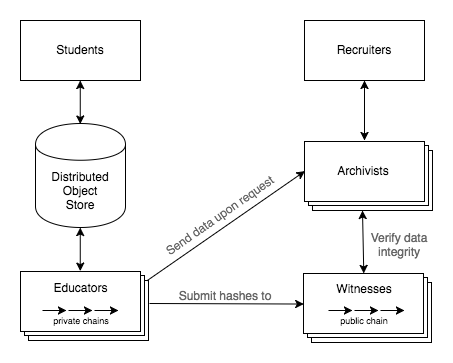
\includegraphics[width=0.8\textwidth]{entities}
\caption{Key entities of the Disciplina platform}
\label{fig:entities}
\end{figure}

The private layer is maintained by each Educator independently of others. Educators can be either large educational institutes, capable of running their own nodes, or some trusted party that runs the chain for the self-employed teachers and small institutions. This layer contains the personalized information on the interactions between the students and the Educator. All the interactions, such as receiving an assignment, submitting solutions, or being graded, are treated as transactions in the private chain.

Students get access to the platform through web and mobile applications. Using the applications they choose Educators, enroll in courses, get assignments and submit solutions. The scores and the criteria of whether the Student has finished the course successfully are determined by the Educator. The education process from the platform’s perspective is as follows:
\begin{enumerate}
\item A Student chooses an Educator and a course that she wants to enroll in
\item If the course is offered on a pre-paid basis, the Student uses her app to pay the fee.
\item The Student’s application communicates with the Educators’ software and performs the key exchange.
\item During the course, the Educator provides assignments that the Student has to complete in order to get the score. The Educator’s software encrypts the assignments with the key the parties agreed upon, and puts it into a distributed Object Store.
\item The Student acquires the assignment, completes it and puts the solution to the Object Store (which is encrypted as well).
\item The Educator then grades the solution and transfers the artifacts along with the score to the blockchain.
\item Upon the completion of the course, the Student acquires a final score based on the scores she got for her assignments. This final score is also added to the Educator’s chain.
\end{enumerate}

Making the Educators' chains private opens the possibility for Educators to tamper with the data in their chains. To overcome this issue and make the private transactions publicly verifiable, we introduce the second, public, layer of the blockchain. The public part of the network consists
of Witnesses – the special entities that witness the fact that a private block was produced by an  Educator.
They do so by writing the authentication information of a private block into the public chain, which is used in the future by an arbitrary Verifier to substantiate a proof of transaction inclusion given to it by a Student or an Educator. Witnesses also process public information issued by the Educators, such as announcements that an Educator has started or stopped offering a course in a particular discipline. The Witnesses agree on which public blocks are valid using the specified consensus rules.

Archivists are entities that provide an interface for the Recruiters to communicate with the platform. The Archivists act like a bridge between the Recruiters and the Educators: they choose the institutes that are relevant for the particular request, orchestrate the data disclosure and provide the evidence on the validity of that data. They obtain this evidence by communicating with Witnesses and comparing the headers of the private data blocks with the headers stored in the public Witnesses' chain.
